%------------------------------------------------------------------------------
%Description       : DDMoRe WP7.2.1 First Technical Specification for the Model
%                                   Repository Infrastructure - Introduction 
%Author            : Mihai Glonț <mglont@ebi.ac.uk>
%Organization      : EMBL-EBI
%                    Wellcome Trust Genome Campus
%                    Hinxton
%                    Cambridge
%                    United Kingdom
%------------------------------------------------------------------------------
\section{Introduction}
\label{introduction}
This document describes the technical infrastructure required by the \ddmore Model Repository. The guidelines herein apply not only to the public Repository, but also to any private instances of it.

\subsection{Context}
\label{context}
In a world where inefficient data and knowledge sharing between academia, pharmaceutical companies and regulatory bodies hinders the development of better medicines, the Drug Disease Model Resources project (\ddmore) -- a Europe-wide project funded by Innovative Medicines Initiative Joint Undertaking -- seeks to create an environment governed by standards that addresses these shortcomings. Specifically, the \ddmore consortium will develop a common definition language for data, models and work flows, as well as a standard for storing and exchanging \glspl{model} and associated metadata\cite{ddmore:dow}.

A significant role within the project is Task 7.2 -- the \ddmore Model Repository. Encompassing non-competitive drug-development models, as well as components created by the scientific community, it will become a centralised worldwide public resource for curated models in key therapeutic areas, promoting knowledge reuse in the field of drug discovery. 

Task 7.2 is closely linked with other deliverables of \ddmore. For instance, the pre-competitive models that will populate the Model Repository initially will be provided by WP1. The models will be encoded in an XML-based format developed by WP4 and the Repository will employ the software library created by Task 2.3 for their manipulation. Finally, the published models stored in the \ddmore Model Repository will be showcased in the Public Instance of the Modelling Framework generated by Task 7.1.

A \ddmore user may interact with the Model Repository using the means depicted in Figure~\ref{fig:userInteraction}. As such, one may access the Repository directly -- through the web-based user interface -- or indirectly, via the Modelling Interoperability Framework, that uses the Task Execution Language (TEL) and the software library created in WP2.3 to access and store models in the \ddmore Model Repository. 

\begin{figure}[htb]
\centering
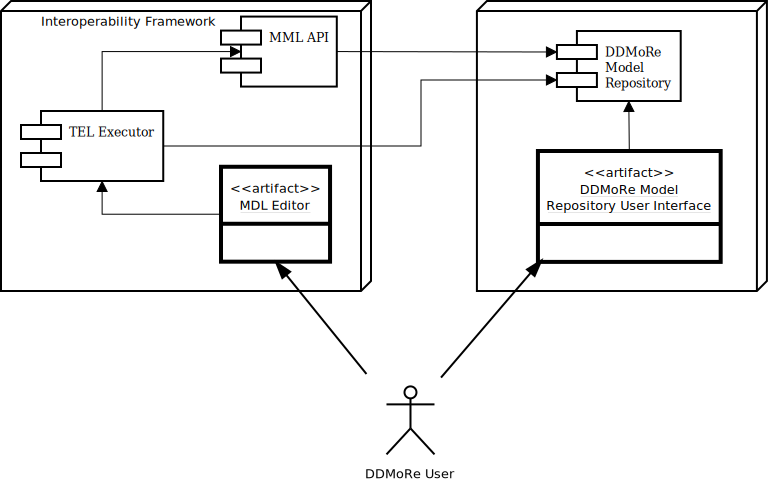
\includegraphics[width=0.75\linewidth]{img/UserInteraction}
\caption{Overview of the interaction between \ddmore users and the Model Repository.}
\label{fig:userInteraction}
\end{figure}
